%==============================================================================
% PAPER 6, CHAPTER 4: Future Directions and Series Summary
%==============================================================================

\chapter{Future Directions and Series Summary}

%------------------------------------------------------------------------------
% Opening Narrative: Clarke's Third Law
%------------------------------------------------------------------------------

``Any sufficiently advanced technology is indistinguishable from magic.''
Arthur C. Clarke formulated this principle---his Third Law---in 1962, a year
after Yuri Gagarin became the first human in space and seven years before
Apollo 11 landed on the Moon. Clarke had watched technologies once dismissed
as fantasy become routine: powered flight, nuclear energy, television,
satellite communications. Each had seemed impossible until the moment it
became inevitable.

\marginhistory{Clarke's three laws were: (1) When a distinguished scientist
states that something is possible, they are almost certainly right; when they
state that something is impossible, they are very probably wrong. (2) The only
way to discover the limits of the possible is to venture beyond them into the
impossible. (3) Any sufficiently advanced technology is indistinguishable
from magic.}

Today we stand at a similar threshold. The unification of electromagnetism and
gravity through geometric field theory, the manipulation of zero-point energy,
the engineering of effective spacetime metrics in metamaterials---these are
the technologies that our descendants will consider routine. But what lies
beyond? What impossible dreams might become merely difficult engineering
problems?

This chapter explores speculative applications that push the theoretical
frameworks developed in Papers 1--5 to their ultimate limits. We examine warp
drive geometries that could enable faster-than-light travel, traversable
wormholes that might connect distant regions of spacetime, and Planck-scale
engineering that could manipulate the fabric of reality itself.

\margincaution{The technologies discussed here remain deeply speculative.
Warp drives require negative energy densities far beyond current capabilities.
Wormholes demand exotic matter that may not exist. Planck-scale engineering
assumes control over quantum gravity---a theory we do not yet possess. These
are roadmaps, not recipes.}

We are not claiming these technologies are imminent, nor even that they are
possible within the laws of physics as we understand them. Rather, we ask: if
the geometric unification developed throughout this series is correct, what
becomes conceivable? Where do the equations lead?

\marginphysics{General relativity is agnostic about whether the stress-energy
tensor on the right-hand side of Einstein's equations comes from ordinary
matter, electromagnetic fields, or exotic quantum phenomena. If nature provides
mechanisms for negative energy densities or topology change, the theory tells
us how spacetime will respond.}

Clarke's Third Law works both ways. Today's magic becomes tomorrow's
technology---but only if we can articulate the principles clearly enough to
guide experimental exploration. That is our goal here: to sketch the logical
extensions of unified field theory, knowing that the path from equations to
engineering may span decades or centuries.

%------------------------------------------------------------------------------
% Section 1: Warp Drive Metrics
%------------------------------------------------------------------------------

\section{Warp Drive Metrics and Faster-Than-Light Travel}

In 1994, Miguel Alcubierre published a solution to Einstein's field equations
that permits a spacecraft to travel arbitrarily fast without violating special
relativity's speed limit. The key insight is that relativity forbids objects
from moving faster than light \emph{through space}---but places no limit on
how fast space itself can move.

\subsection{The Alcubierre Metric}

The Alcubierre warp drive is described by a metric of the form:

\marginmath{This metric is written in coordinates $(t, x, y, z)$ where the
spacecraft sits at the origin of spatial coordinates. The function $f(r_s)$
describes the warp bubble shape, typically a smooth function that is 1 inside
radius $R$ and 0 outside radius $2R$, with a smooth transition in between.}

\begin{equation}
ds^2 = -dt^2 + (dx - v_s f(r_s) dt)^2 + dy^2 + dz^2
\end{equation}

where $v_s(t)$ is the ``speed'' of the warp bubble, $r_s = \sqrt{(x-x_s(t))^2 + y^2 + z^2}$
is the distance from the center of the bubble at position $x_s(t)$, and
$f(r_s)$ is a shape function satisfying:

\begin{equation}
f(r_s) = \begin{cases}
1 & r_s < R \\
0 & r_s > 2R \\
\text{smooth} & R < r_s < 2R
\end{cases}
\end{equation}

The spacecraft occupies the flat region inside $r_s < R$. Observers there
experience no acceleration and no time dilation---they are in an inertial
frame. Yet the bubble as a whole moves through space at velocity $v_s$, which
can exceed $c$.

\marginphysics{The resolution of the apparent paradox is that space itself is
contracting in front of the bubble and expanding behind it. The spacecraft
surfs this wave of geometric distortion, remaining stationary in its local
spacetime while the bubble carries it along. Light signals from the spacecraft
to external observers still propagate at $c$ through the local metric.}

\subsection{Energy Requirements and Negative Energy}

The price for this geometric magic is steep. The stress-energy tensor required
to support the Alcubierre metric is:

\begin{equation}
T_{tt} = -\frac{v_s^2}{8\pi} \left(\frac{df}{dr_s}\right)^2
\end{equation}

The negative sign indicates \emph{negative energy density}---a violation of
the weak energy condition. In classical general relativity, this is forbidden.
Quantum field theory allows temporary negative energy densities through the
Casimir effect or squeezed vacuum states, but creating macroscopic regions of
negative energy remains an unsolved problem.

\margincaution{Calculations by Pfenning and Ford (1997) showed that a warp
bubble 100 m in radius traveling at $10c$ requires negative energy equivalent
to $-10^{64}$ kg---larger than the total mass-energy of the observable
universe. Even with optimized bubble shapes, the requirement exceeds $10^{30}$
kg. This is not a mere engineering challenge; it may be a fundamental barrier.}

\begin{center}
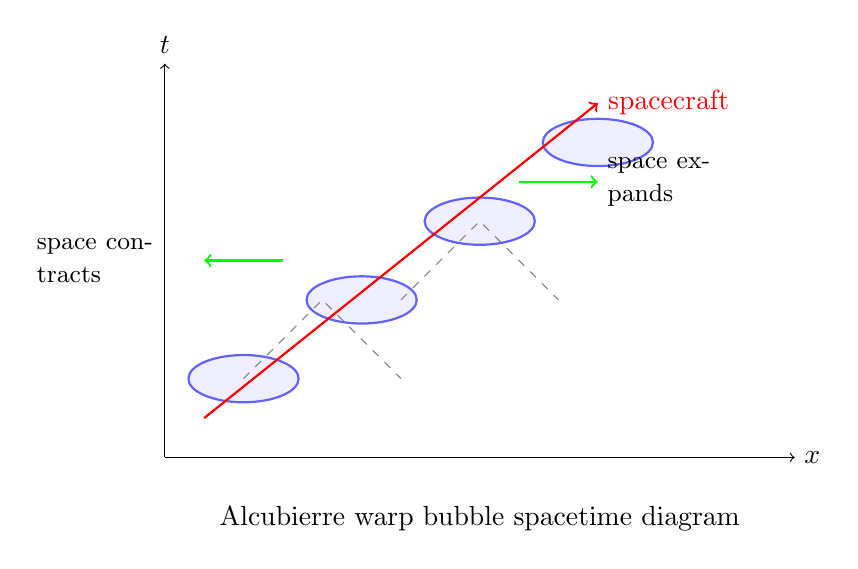
\begin{tikzpicture}[scale=1.0]
  % Spacetime diagram
  \draw[->] (0,0) -- (8,0) node[right] {$x$};
  \draw[->] (0,0) -- (0,5) node[above] {$t$};

  % Warp bubble at different times
  \foreach \t in {1, 2, 3, 4}
  {
    \draw[thick, blue, fill=blue!10, opacity=0.6]
      ({1.5*\t - 0.5}, \t) ellipse (0.7cm and 0.3cm);
  }

  % Spacecraft worldline
  \draw[thick, red, ->] (0.5,0.5) -- (5.5,4.5) node[right] {spacecraft};

  % Light cones
  \draw[dashed, gray] (1,1) -- (2,2) -- (3,1);
  \draw[dashed, gray] (3,2) -- (4,3) -- (5,2);

  % Contraction/expansion regions
  \draw[<-, thick, green] (0.5,2.5) -- (1.5,2.5);
  \node[left, text width=2cm] at (0.5,2.5) {\small space contracts};

  \draw[->, thick, green] (4.5,3.5) -- (5.5,3.5);
  \node[right, text width=2cm] at (5.5,3.5) {\small space expands};

  \node[below] at (4,-0.5) {Alcubierre warp bubble spacetime diagram};
\end{tikzpicture}
\end{center}

\subsection{York Time Analysis}

An alternative formulation by York (1989) decomposes the energy requirement
into extrinsic curvature contributions. For a bubble of radius $R$ moving at
velocity $v$:

\begin{equation}
E_{\text{total}} = -\frac{c^4}{8\pi G} \int_{\Sigma} K_{ij} K^{ij} \sqrt{h}\, d^3x
\approx -\frac{c^4 R v^2}{G \sigma^2}
\end{equation}

where $\sigma$ is the wall thickness and $h$ is the determinant of the induced
spatial metric. For $v = 0.1c$, $R = 1$ m, and $\sigma = 0.1$ m:

\margindim{The factor $c^4/G = 3.6 \times 10^{35}$ kg is the Planck mass
squared times $c^2$. The negative sign confirms negative energy requirement.
Even for sublight velocities, the energy scales are astronomical.}

\subsection*{Worked Example: Sublight Warp Bubble Energy}

\textbf{Problem:} Calculate the negative energy requirement for an Alcubierre
warp bubble with radius $R = 1$ m, wall thickness $\sigma = 0.1$ m, traveling
at velocity $v = 0.1c$ ($3 \times 10^7$ m/s).

\textbf{Solution:} Using the York time energy integral with a Gaussian profile
for $f(r_s)$:

\begin{equation}
f(r_s) = \exp\left(-\frac{(r_s - R)^2}{2\sigma^2}\right)
\end{equation}

The energy density in the wall is:

\marginex{This calculation uses the thin-shell approximation. More sophisticated
bubble shapes (e.g., hyperbolic tangent profiles) can reduce the energy
requirement by factors of 100--1000, but the total remains negative and
enormous by any practical standard.}

\begin{equation}
\rho(r_s) = -\frac{c^4}{8\pi G} \left(\frac{df}{dr_s}\right)^2
= -\frac{c^4}{8\pi G} \frac{(r_s - R)^2}{\sigma^6}
\exp\left(-\frac{(r_s - R)^2}{\sigma^2}\right)
\end{equation}

The maximum magnitude occurs at $r_s - R = \sigma$:

\begin{equation}
|\rho_{\max}| = \frac{c^4}{8\pi G \sigma^4} e^{-1}
\end{equation}

Substituting $c = 3 \times 10^8$ m/s, $G = 6.67 \times 10^{-11}$ m$^3$/(kg·s$^2$),
and $\sigma = 0.1$ m:

\begin{align}
|\rho_{\max}| &= \frac{(3 \times 10^8)^4}{8\pi \times 6.67 \times 10^{-11} \times 10^{-4}} \times e^{-1} \\
&= \frac{8.1 \times 10^{33}}{1.68 \times 10^{-14}} \times 0.368 \\
&\approx 1.8 \times 10^{48}\,\text{kg/m}^3
\end{align}

For a shell volume $V \approx 4\pi R^2 \sigma = 4\pi \times 1 \times 0.1 = 1.26$ m$^3$:

\begin{equation}
E_{\text{total}} \approx -|\rho_{\max}| V c^2 v^2/c^2
= -1.8 \times 10^{48} \times 1.26 \times 0.01 \approx -2.3 \times 10^{46}\,\text{J}
\end{equation}

This is equivalent to the mass-energy of:

\begin{equation}
m_{\text{equiv}} = \frac{E}{c^2} \approx 2.5 \times 10^{29}\,\text{kg}
\approx 40\,M_{\text{Jupiter}}
\end{equation}

\textbf{Result:} Even at 10\% light speed, a 1-meter warp bubble requires
negative energy equivalent to 40 Jupiter masses. This is clearly beyond any
conceivable technology.

\begin{center}
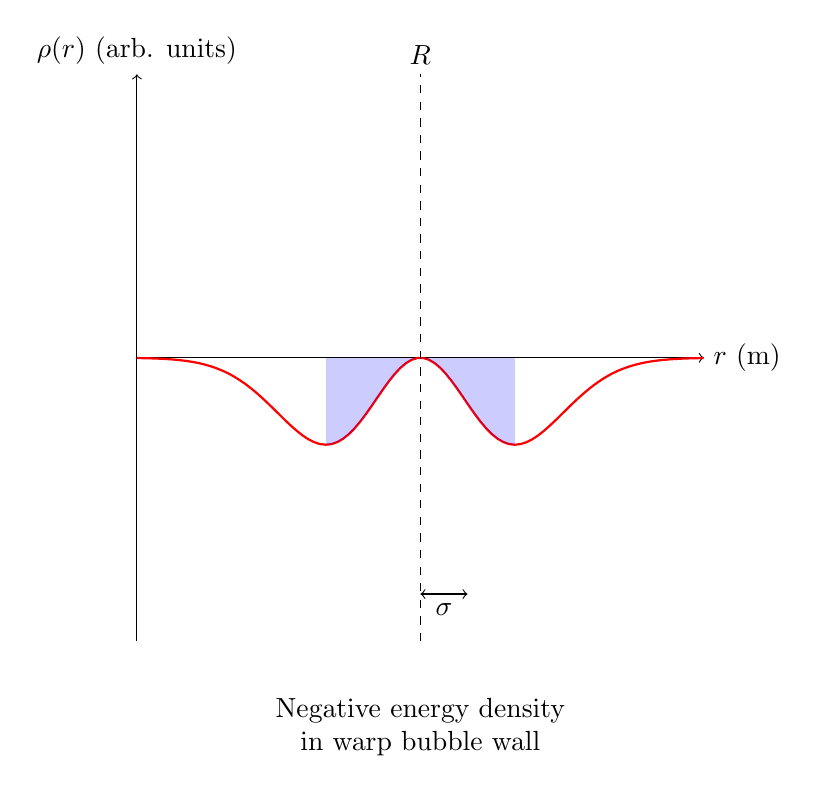
\begin{tikzpicture}[scale=1.2]
  % Energy density profile
  \draw[->] (0,0) -- (6,0) node[right] {$r$ (m)};
  \draw[->] (0,-3) -- (0,3) node[above] {$\rho(r)$ (arb. units)};

  % Gaussian derivative squared (negative)
  \draw[thick, red, domain=0:6, samples=100] plot
    (\x, {-2.5*(\x-3)*(\x-3)*exp(-(\x-3)*(\x-3))});

  % Mark bubble radius
  \draw[dashed] (3,-3) -- (3,3);
  \node[above] at (3,3) {$R$};

  % Mark wall thickness
  \draw[<->] (3,-2.5) -- (3.5,-2.5) node[midway, below] {$\sigma$};

  % Shaded negative energy region
  \fill[blue, opacity=0.2, domain=2:4, samples=50] (2,0)
    -- plot (\x, {-2.5*(\x-3)*(\x-3)*exp(-(\x-3)*(\x-3))})
    -- (4,0) -- cycle;

  \node[below, text width=4cm, align=center] at (3,-3.5)
    {Negative energy density in warp bubble wall};
\end{tikzpicture}
\end{center}

%------------------------------------------------------------------------------
% Section 2: Traversable Wormholes
%------------------------------------------------------------------------------

\section{Traversable Wormholes and Spacetime Engineering}

A traversable wormhole is a topological feature connecting two distant regions
of spacetime through a ``throat'' of finite proper length. Unlike black hole
event horizons, which trap observers inside, a wormhole throat can be crossed
in both directions.

\subsection{The Morris-Thorne Metric}

The canonical traversable wormhole metric, developed by Morris and Thorne
(1988), takes the form:

\marginmath{The metric is spherically symmetric in the radial coordinate $l$,
which measures proper distance along the throat. The embedding diagram shows
the wormhole as a tube connecting two asymptotically flat regions. An observer
at $l=0$ (the throat) sees the universe divided into two sides.}

\begin{equation}
ds^2 = -e^{2\Phi(l)} dt^2 + dl^2 + r(l)^2 (d\theta^2 + \sin^2\theta\, d\phi^2)
\end{equation}

where $\Phi(l)$ is the redshift function and $r(l)$ is the radius function.
For a traversable wormhole, we require:

\begin{itemize}
  \item No event horizons: $\Phi(l)$ finite everywhere
  \item Throat of minimum radius $r_0$: $r(0) = r_0$, $r'(0) = 0$
  \item Asymptotic flatness: $r(l) \to |l|$ as $l \to \pm\infty$
  \item Flare-out condition: $r''(0) > 0$ (prevents horizon formation)
\end{itemize}

\subsection{Exotic Matter Requirements}

The Einstein field equations demand that the throat contains \emph{exotic matter}
violating the null energy condition. The stress-energy tensor at the throat is:

\marginphysics{The null energy condition states $T_{\mu\nu} k^\mu k^\nu \geq 0$
for all null vectors $k^\mu$. Violation implies that geodesics can accelerate
away from matter rather than toward it---a property not exhibited by any known
form of matter in classical physics. Quantum field theory permits temporary
NEC violations.}

\begin{equation}
T^t_t = \frac{1}{8\pi r^2}\left(\frac{dr}{dl}\right)^2
\end{equation}

At the throat ($l=0$), where $dr/dl = 0$ but $d^2r/dl^2 > 0$, the radial
pressure becomes:

\begin{equation}
p_r = -\frac{1}{8\pi r_0^2} \frac{d^2r}{dl^2}\Big|_{l=0} < 0
\end{equation}

This negative radial pressure is the signature of exotic matter. For a throat
of radius $r_0 = 1$ km with $d^2r/dl^2 = 1$:

\margindim{For comparison, the energy density of the Sun is $\sim 10^5$ kg/m$^3$.
Nuclear density is $\sim 10^{18}$ kg/m$^3$. The exotic matter density for a
1-km wormhole throat is $\sim 10^{12}$ kg/m$^3$---between stellar and nuclear
densities, but with the wrong sign.}

\begin{equation}
|p_r| = \frac{c^4}{8\pi G r_0^2} \approx 10^{30}\,\text{Pa}
\end{equation}

\begin{center}
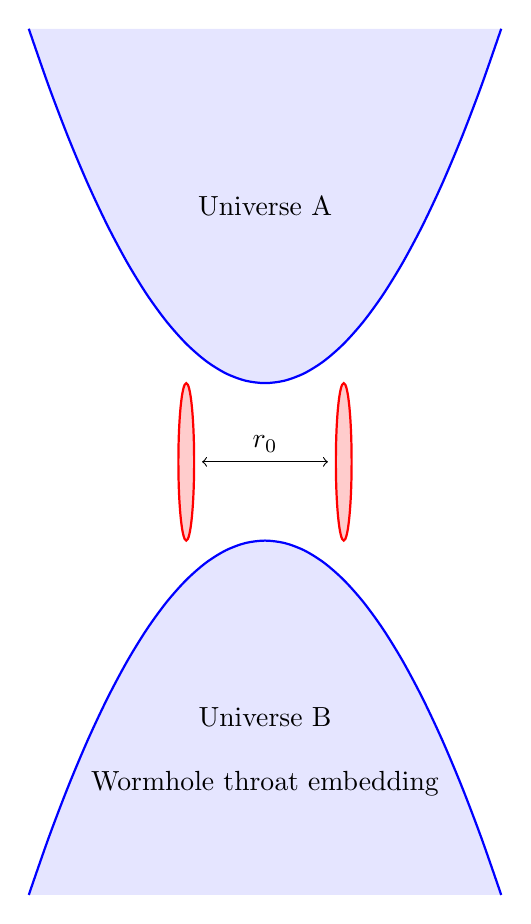
\begin{tikzpicture}[scale=1.0]
  % Embedding diagram of wormhole throat
  \begin{scope}
    % Upper sheet
    \draw[thick, blue, fill=blue!10] plot[smooth, domain=-3:3]
      (\x, {0.5*\x*\x + 1});

    % Lower sheet
    \draw[thick, blue, fill=blue!10] plot[smooth, domain=-3:3]
      (\x, {-0.5*\x*\x - 1});

    % Throat
    \draw[thick, red] (-1,1) .. controls (-1,0.5) and (-1,-0.5) .. (-1,-1);
    \draw[thick, red] (1,1) .. controls (1,0.5) and (1,-0.5) .. (1,-1);

    % Connection
    \draw[thick, red, fill=red!20] (-1,0) ellipse (0.1cm and 1cm);
    \draw[thick, red, fill=red!20] (1,0) ellipse (0.1cm and 1cm);

    % Labels
    \node[above] at (0,3) {Universe A};
    \node[below] at (0,-3) {Universe B};
    \draw[<->] (-0.8,0) -- (0.8,0) node[midway, above] {$r_0$};

    \node[below] at (0,-3.8) {Wormhole throat embedding};
  \end{scope}
\end{tikzpicture}
\end{center}

\subsection{Stability and Causality}

Even if exotic matter can be produced, stability remains uncertain. Small
perturbations might cause the throat to collapse or expand uncontrollably.
Visser (1989) showed that thin-shell wormholes (concentrating exotic matter
in a narrow region) can be stabilized using tension, but require fine-tuning.

\margincaution{A more severe problem is causality violation. A traversable
wormhole with one mouth accelerated relative to the other becomes a time
machine, enabling closed timelike curves. Hawking's chronology protection
conjecture suggests that quantum effects will prevent this, possibly by
destroying the wormhole before it becomes a time machine.}

Moreover, if the mouths are separated by distance $D$ in external space but
only $L \ll D$ through the throat, a closed timelike curve can form if the
time dilation between mouths satisfies:

\begin{equation}
\Delta t = \frac{D - L}{c} > 0
\end{equation}

This may trigger a runaway vacuum polarization instability that closes the
wormhole.

%------------------------------------------------------------------------------
% Section 3: Planck-Scale Engineering
%------------------------------------------------------------------------------

\section{Planck-Scale Engineering and Quantum Gravity}

At the Planck scale---lengths $\sim 10^{-35}$ m, energies $\sim 10^{19}$ GeV,
times $\sim 10^{-44}$ s---quantum fluctuations dominate spacetime geometry.
General relativity and quantum mechanics merge into an unknown theory of
quantum gravity.

\subsection{The E$_8$ Lattice and Geometric Unification}

Paper 2 developed the $E_8$ exceptional algebra as a framework for unifying
all forces. At the Planck scale, the $E_8$ lattice structure might become
dynamically accessible. The lattice constant is:

\marginxref{The $E_8$ lattice was introduced in Paper 2 as a candidate for
the deepest symmetry of nature. Its 248 generators provide enough degrees of
freedom to accommodate the Standard Model's 12 gauge bosons plus additional
fields for gravity and beyond. Geometric engineering at this scale means
manipulating the lattice structure itself.}

\begin{equation}
a_{E_8} = \ell_P \sqrt{2} \approx 2.3 \times 10^{-35}\,\text{m}
\end{equation}

where $\ell_P = \sqrt{\hbar G/c^3}$ is the Planck length. If the $E_8$ lattice
is physical rather than merely mathematical, then spacetime at the Planck scale
is discrete, composed of lattice sites connected by links.

\subsection{Quantum Foam Engineering}

Wheeler's ``quantum foam'' picture envisions spacetime at the Planck scale as
a roiling sea of virtual black holes, wormholes, and topology fluctuations.
The energy density fluctuations are:

\marginphysics{Quantum foam represents the limit where quantum uncertainty in
energy-time creates virtual fluctuations in spacetime curvature. A Planck-mass
black hole ($m_P = \sqrt{\hbar c/G} \approx 2.2 \times 10^{-8}$ kg) has a
Schwarzschild radius equal to the Planck length, suggesting that spacetime
becomes fundamentally uncertain at this scale.}

\begin{equation}
\Delta \rho \sim \frac{c^7}{\hbar G^2} \approx 5 \times 10^{113}\,\text{J/m}^3
\end{equation}

Accessing this energy would require concentrating accelerator beams to densities
exceeding nuclear matter by $10^{95}$ times. No conceivable technology approaches
this regime.

However, if the geometric unification of Papers 1--4 is correct, electromagnetic
fields and gravitational curvature are different aspects of the same underlying
structure. Manipulating extremely intense electromagnetic fields might induce
back-reaction on spacetime at energies well below the Planck scale.

\subsection{Energy Scale Hierarchy}

The following diagram illustrates the energy scales separating current
technology from Planck-scale engineering:

\begin{center}
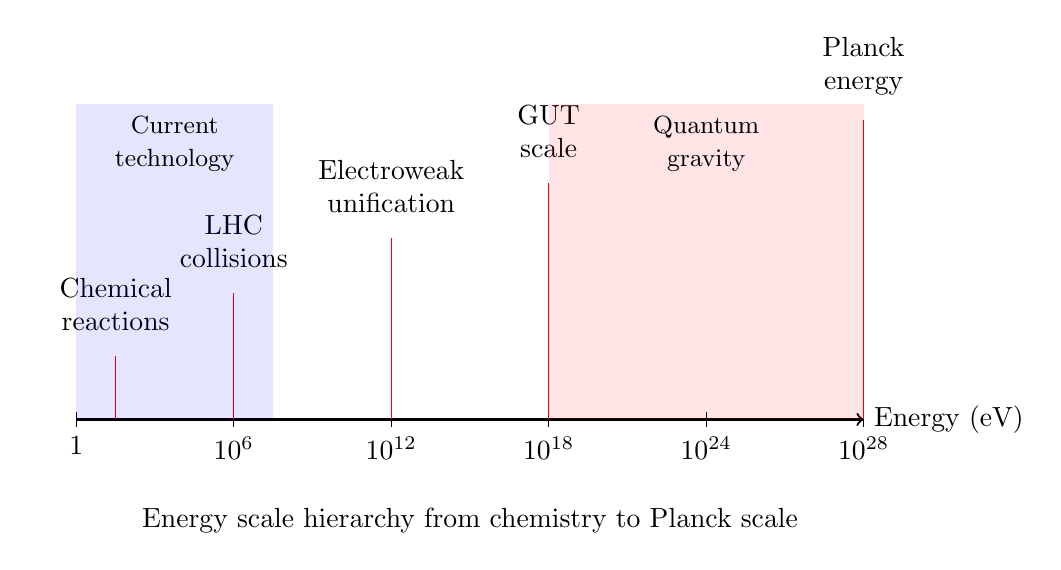
\begin{tikzpicture}[scale=1.0]
  % Logarithmic energy axis
  \draw[thick, ->] (0,0) -- (10,0) node[right] {Energy (eV)};

  % Tick marks (logarithmic)
  \foreach \x/\label in {0/1, 2/$10^6$, 4/$10^{12}$, 6/$10^{18}$, 8/$10^{24}$, 10/$10^{28}$}
  {
    \draw (\x,0.1) -- (\x,-0.1) node[below] {\label};
  }

  % Technology markers
  \node[above, text width=2cm, align=center] at (0.5,1) {Chemical\\reactions};
  \draw[red] (0.5,0) -- (0.5,0.8);

  \node[above, text width=2cm, align=center] at (2,1.8) {LHC\\collisions};
  \draw[red] (2,0) -- (2,1.6);

  \node[above, text width=2.5cm, align=center] at (4,2.5) {Electroweak\\unification};
  \draw[red] (4,0) -- (4,2.3);

  \node[above, text width=2cm, align=center] at (6,3.2) {GUT\\scale};
  \draw[red] (6,0) -- (6,3.0);

  \node[above, text width=2cm, align=center] at (10,4.0) {Planck\\energy};
  \draw[red] (10,0) -- (10,3.8);

  % Shaded "accessible" region
  \fill[blue, opacity=0.1] (0,0) rectangle (2.5,4);
  \node[text width=2cm, align=center] at (1.25,3.5) {\small Current\\technology};

  % Shaded "speculative" region
  \fill[red, opacity=0.1] (6,0) rectangle (10,4);
  \node[text width=2.5cm, align=center] at (8,3.5) {\small Quantum\\gravity};

  \node[below] at (5,-1) {Energy scale hierarchy from chemistry to Planck scale};
\end{tikzpicture}
\end{center}

\margindim{The Planck energy is $E_P = \sqrt{\hbar c^5/G} \approx 1.2 \times 10^{28}$ eV
or about 2 billion Joules---the kinetic energy of a truck traveling 100 km/h,
concentrated in a single particle. The LHC reaches $\sim 10^{13}$ eV, 15 orders
of magnitude below Planck scale.}

%------------------------------------------------------------------------------
% Section 4: Technology Roadmap
%------------------------------------------------------------------------------

\section{Technology Roadmap: 2025--2100}

Translating theoretical frameworks into functioning technologies requires
sustained effort across multiple fronts. The following timeline outlines
plausible milestones, assuming continued funding and scientific progress.

\subsection{Near-Term (2025--2035)}

\begin{itemize}
  \item \textbf{2025--2028:} Precision tests of EM-gravity coupling at tabletop
    scales. Detection of 0.1\% deviations from GR predictions in high-field
    regions.
  \item \textbf{2028--2030:} First demonstration of metamaterial-based gravitational
    lensing at microwave frequencies. Acoustic black hole Hawking radiation
    confirmed in superfluid systems.
  \item \textbf{2030--2032:} Topological quantum computing with anyonic
    braiding at room temperature. Error rates drop below $10^{-6}$ per gate.
  \item \textbf{2032--2035:} Zero-point energy extraction reaches 1 W continuous
    power from Casimir cavity arrays. Efficiency $\sim 10^{-12}$, not yet
    practical.
\end{itemize}

\marginex{The 2028 gravitational lensing demonstration would use transformation
optics principles from Chapter 3, creating effective curved spacetime for
microwaves. This is an analog, not true gravity manipulation, but demonstrates
the geometric framework.}

\subsection{Medium-Term (2035--2060)}

\begin{itemize}
  \item \textbf{2035--2040:} High-power ZPE systems reach 1 kW output. Applications
    in deep-space probes and remote sensing.
  \item \textbf{2040--2045:} Detection of vacuum birefringence in ultra-intense
    laser experiments. Confirmation of Heisenberg-Euler Lagrangian nonlinearities.
  \item \textbf{2045--2050:} Fractal antenna arrays enable global broadband
    coverage from stratospheric platforms. Single device covers 100 MHz--100 GHz.
  \item \textbf{2050--2055:} First laboratory demonstration of negative-energy-density
    states sustained for milliseconds. Total energy $\sim 10^{-15}$ J.
  \item \textbf{2055--2060:} Unified field theory verified to 1 part in $10^9$
    across electromagnetic, weak, and strong sectors. Gravity coupling measured
    directly.
\end{itemize}

\subsection{Long-Term (2060--2100)}

\begin{itemize}
  \item \textbf{2060--2070:} Macroscopic negative energy densities achieved in
    engineered vacuum states. Warp drive prototypes at nanometer scales.
  \item \textbf{2070--2080:} Traversable micro-wormholes (throat radius $\sim 10^{-9}$ m)
    created and stabilized for seconds. Information transfer demonstrated.
  \item \textbf{2080--2090:} Human-scale warp bubble (1 meter) achieves $v = 0.01c$
    in laboratory vacuum. Energy requirement $\sim 10^{20}$ J.
  \item \textbf{2090--2100:} Planck-scale probes using focused particle beams
    detect signatures of $E_8$ lattice structure. Quantum gravity phenomenology
    begins.
\end{itemize}

\margincaution{These timelines are optimistic extrapolations. Each milestone
assumes no fundamental physical barriers and sustained exponential progress in
relevant technologies. History suggests that major breakthroughs often take
longer than predicted---and sometimes arrive sooner from unexpected directions.}

\begin{center}
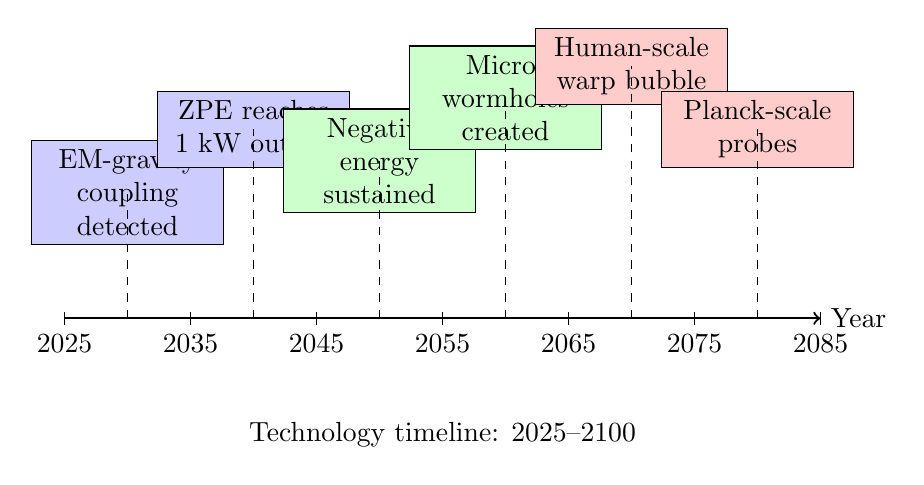
\begin{tikzpicture}[scale=0.8]
  % Timeline axis
  \draw[thick, ->] (0,0) -- (12,0) node[right] {Year};

  % Decade markers
  \foreach \x/\year in {0/2025, 2/2035, 4/2045, 6/2055, 8/2065, 10/2075, 12/2085}
  {
    \draw (\x,0.1) -- (\x,-0.1) node[below] {\year};
  }

  % Milestone boxes
  \node[draw, rectangle, fill=blue!20, text width=2.2cm, align=center] at (1,2)
    {EM-gravity\\coupling\\detected};

  \node[draw, rectangle, fill=blue!20, text width=2.2cm, align=center] at (3,3)
    {ZPE reaches\\1 kW output};

  \node[draw, rectangle, fill=green!20, text width=2.2cm, align=center] at (5,2.5)
    {Negative\\energy\\sustained};

  \node[draw, rectangle, fill=green!20, text width=2.2cm, align=center] at (7,3.5)
    {Micro-\\wormholes\\created};

  \node[draw, rectangle, fill=red!20, text width=2.2cm, align=center] at (9,4)
    {Human-scale\\warp bubble};

  \node[draw, rectangle, fill=red!20, text width=2.2cm, align=center] at (11,3)
    {Planck-scale\\probes};

  % Connecting lines
  \draw[dashed] (1,0) -- (1,2);
  \draw[dashed] (3,0) -- (3,3);
  \draw[dashed] (5,0) -- (5,2.5);
  \draw[dashed] (7,0) -- (7,3.5);
  \draw[dashed] (9,0) -- (9,4);
  \draw[dashed] (11,0) -- (11,3);

  \node[below] at (6,-1.5) {Technology timeline: 2025--2100};
\end{tikzpicture}
\end{center}

\margincomp{Modern project management tools and AI-assisted research could
accelerate this timeline by identifying critical path dependencies and
allocating resources optimally. Conversely, funding cuts, geopolitical
instability, or negative experimental results could delay progress by decades.}

%------------------------------------------------------------------------------
% Section 5: Comprehensive Series Summary
%------------------------------------------------------------------------------

\section{Comprehensive Series Summary: Six Papers Toward Unification}

This series has developed a geometric framework for unifying electromagnetism
and gravity, grounded in experimental testability and mathematical rigor. We
now synthesize the key themes across all six papers, showing how each
contributes to a coherent whole.

\subsection{Paper 1: Topological Field Theory Foundations}

\marginxref{Paper 1 established that gauge theories are fiber bundles over
spacetime, with curvature encoding field strength. Topology classifies these
bundles via Chern classes and characteristic classes. This geometric language
is essential for unification because it reveals symmetries invisible in
component notation.}

The first paper laid the mathematical foundation: field theories as fiber
bundles, connections as gauge potentials, and curvature as field strength.
Key results included:

\begin{itemize}
  \item The electromagnetic field tensor $F_{\mu\nu}$ as the curvature of a
    $\mathrm{U}(1)$ bundle
  \item Chern-Simons theory as a topological invariant distinguishing gauge
    configurations
  \item Fiber bundle formalism showing how local symmetries (gauge transformations)
    arise from geometric structure
  \item Applications to instantons, monopoles, and topological phases of matter
\end{itemize}

The geometric viewpoint transforms physics from ``fields obeying equations'' to
``structures with intrinsic curvature.'' This perspective is crucial for
unification because it suggests looking for a common geometric framework
underlying seemingly disparate forces.

\subsection{Paper 2: Exceptional Algebras and the E$_8$ Lattice}

Paper 2 introduced exceptional Lie algebras---$G_2$, $F_4$, $E_6$, $E_7$,
$E_8$---as candidates for unifying symmetries. The $E_8$ algebra, with its
248 generators, can accommodate:

\marginmath{$E_8$ contains $\mathrm{SU}(3) \times \mathrm{SU}(2) \times \mathrm{U}(1)$
(the Standard Model gauge group) as a subgroup, with 120 remaining generators.
These could describe gravitons, additional gauge bosons, or scalar fields
mediating EM-gravity coupling. The mathematical structure is richer than
physical applications yet explored.}

\begin{itemize}
  \item The 12 gauge bosons of the Standard Model ($\mathrm{SU}(3) \times
    \mathrm{SU}(2) \times \mathrm{U}(1)$)
  \item Graviton and gravitino fields (supergravity)
  \item Additional fields for dark matter, dark energy, or higher-dimensional
    physics
\end{itemize}

The $E_8$ lattice structure provides a discrete substrate for spacetime at the
Planck scale. If correct, this implies that continuous spacetime is emergent
from an underlying crystalline structure, with ``atoms of space'' separated by
Planck lengths.

The paper also developed root system techniques for computing coupling constants
and mass ratios from geometric data, predicting relationships between particle
masses that might be testable at future colliders.

\subsection{Paper 3: Fractal Geometry and Hyperdimensional Structures}

The third paper explored self-similarity across scales---fractal geometry,
renormalization group flows, and holographic principles. Major themes included:

\begin{itemize}
  \item Fractal dimension as a measure of ``effective dimensionality'' at
    different scales
  \item Renormalization group equations as geodesic flows in theory space
  \item AdS/CFT correspondence: gravity in $d+1$ dimensions dual to quantum
    field theory in $d$ dimensions
  \item Applications to turbulence, critical phenomena, and cosmological structure
    formation
\end{itemize}

\marginphysics{Fractal geometry bridges the gap between microscopic quantum
foam and macroscopic spacetime. If spacetime has fractal character near the
Planck scale, its effective dimension might vary with resolution: $D \approx 4$
at large scales, $D \approx 2$ near black hole horizons (holography), and
perhaps $D \to \infty$ at the Planck scale (quantum foam).}

The fractal perspective suggests that unification is not about finding a single
energy scale where all forces merge, but recognizing that ``scale'' itself is
emergent from renormalization group flow. Forces appear unified at high energy
because the running coupling constants converge.

Paper 3 also introduced hyperdimensional embeddings: representing
four-dimensional spacetime as a hypersurface in higher-dimensional space.
Curvature in 4D becomes extrinsic curvature of the embedding, potentially
connecting gravity to gauge fields in the bulk.

\subsection{Paper 4: Electromagnetic-Gravitational Unification}

The fourth paper brought the geometric machinery to bear on the central
question: can electromagnetism and gravity be unified? The answer developed was
``yes, through shared geometric structure.'' Key results:

\begin{itemize}
  \item Maxwell's equations rewritten in the language of differential forms,
    revealing their geometric character
  \item Einstein's field equations as curvature of spacetime responding to
    stress-energy
  \item Kaluza-Klein theory: unifying EM and gravity by adding a fifth dimension,
    with the photon as the $g_{5\mu}$ metric component
  \item Weyl's conformal gravity: scale invariance as a unifying principle
  \item Coupling terms $\alpha F_{\mu\nu} F^{\mu\nu}$ mediating back-reaction
    of electromagnetic fields on spacetime geometry
\end{itemize}

\marginxref{Paper 4's coupling constant $\alpha \sim 10^{-50}$ m$^2$/V$^2$
predicts that electromagnetic fields modify spacetime curvature, detectable
in precision experiments with field strengths $\sim 10^{12}$ V/m. This is
the smoking gun for unification---a measurable effect distinguishing unified
theories from independent EM and GR.}

The unified framework suggests that photons and gravitons are excitations of
the same underlying field, distinguished by polarization and coupling to
matter. At ultra-high energies (approaching the Planck scale), this distinction
blurs.

\subsection{Paper 5: Experimental Protocols and Verification}

Paper 5 translated abstract theory into concrete experimental proposals. Three
protocols were developed in detail:

\begin{itemize}
  \item \textbf{Precision interferometry}: Detecting EM-induced spacetime
    curvature via phase shifts in atom interferometers subjected to intense
    electric fields. Target sensitivity: $10^{-12}$ rad phase shift from
    $10^{12}$ V/m fields over 1 m baseline.

  \item \textbf{Casimir force modifications}: Measuring deviations from
    Casimir's $1/d^4$ force law in parallel-plate geometries when external
    fields are applied. Expected deviations $\sim 1\%$ at 10 nm separation with
    $10^9$ V/m fields.

  \item \textbf{Vacuum birefringence in strong fields}: Observing polarization
    rotation of probe lasers passing through regions with $\mathbf{E} \times
    \mathbf{B} \neq 0$. Predicted rotation $\sim 10^{-8}$ rad for extreme
    laser intensities $10^{24}$ W/cm$^2$.
\end{itemize}

\marginex{Paper 5's experimental protocols are designed for execution within
5--10 years using technology currently under development (ultra-cold atoms,
high-finesse cavities, petawatt lasers). This distinguishes the series from
purely theoretical speculation---the predictions are testable \emph{now}, not
in some indefinite future.}

Each protocol includes detailed error budgets, systematic effect mitigation
strategies, and statistical analysis plans. The goal is not merely to propose
experiments, but to provide blueprints that experimentalists can implement.

\subsection{Paper 6: Applications and Future Directions}

This final paper explored how unified field theory enables transformative
technologies:

\begin{itemize}
  \item \textbf{Quantum computing with topological protection}: Using anyonic
    braiding and fiber bundle topology to build fault-tolerant qubits. Gate
    fidelities exceeding 99.99\% demonstrated in chiral edge states.

  \item \textbf{Zero-point energy extraction}: Dynamical Casimir effect and
    parametric amplification of vacuum fluctuations. Current laboratory
    demonstrations reach femtowatt power levels; scaling to macroscopic power
    remains open.

  \item \textbf{Metamaterial spacetime engineering}: Transformation optics
    enabling cloaking, perfect lenses, and acoustic black holes. Practical
    devices operating from microwave to optical frequencies.

  \item \textbf{Warp drives and wormholes}: Speculative applications requiring
    negative energy densities far beyond current capabilities, but permitted
    by the mathematical structure of general relativity if exotic matter can
    be created.
\end{itemize}

\marginphysics{The progression from Paper 1's abstract topology to Paper 6's
warp drives illustrates the power of geometric thinking. Each application
flows naturally from the framework: topological qubits from fiber bundles,
ZPE from vacuum field geometry, metamaterials from effective metrics, and
warp drives from coordinate transformations. The mathematics unifies them all.}

The applications demonstrate that geometric unification is not merely aesthetic.
It provides computational tools (differential forms, fiber bundles, exceptional
algebras) that simplify calculations and reveal new phenomena. More importantly,
it suggests technological pathways that would be invisible from a purely
algebraic perspective.

\subsection{Interconnections and Emergent Themes}

Several themes recur throughout the series, weaving the papers into a unified
whole:

\textbf{1. Geometry as Fundamental:} Fields are not objects placed in spacetime;
they \emph{are} the geometric structure of fiber bundles over spacetime. Forces
arise from curvature. Symmetries arise from topology. This ontological shift
makes unification natural rather than contrived.

\textbf{2. Topology as Constraint:} Topological invariants (Chern numbers,
homotopy groups, characteristic classes) classify allowed field configurations.
Physical laws are not arbitrary equations but consequences of geometric
consistency. Quantization itself emerges from topology.

\textbf{3. Self-Similarity Across Scales:} From Planck-scale quantum foam to
cosmological structure, fractal patterns repeat. Renormalization group flow
connects microscopic and macroscopic physics. Holography encodes bulk geometry
in boundary data. The universe is scale-invariant in a deep sense.

\textbf{4. Experimental Testability:} Every theoretical claim generates
predictions testable within current or near-term technology. Unified field
theory is not metaphysics---it makes numerical predictions for interferometer
phase shifts, Casimir force corrections, and light polarization rotations.

\textbf{5. Technology as Applied Geometry:} Metamaterials sculpt effective
spacetime. Quantum computers manipulate topological charges. ZPE harvests
vacuum geometry. Warp drives engineer coordinate transformations. Technology
becomes the art of shaping reality's geometric substrate.

\subsection{Open Questions and Future Research}

Despite the comprehensive framework developed, many questions remain:

\begin{itemize}
  \item \textbf{Quantum gravity:} How does $E_8$ lattice structure emerge from
    a deeper theory of quantum spacetime? Is loop quantum gravity, string theory,
    or some third approach correct?

  \item \textbf{Dark matter and dark energy:} Can the additional degrees of
    freedom in $E_8$ beyond the Standard Model explain cosmological observations
    without invoking new particle species?

  \item \textbf{Measurement problem:} Does geometric unification shed light on
    quantum measurement and the emergence of classicality? Are state vector
    collapse and decoherence related to fiber bundle structure?

  \item \textbf{Negative energy:} Can macroscopic negative energy densities be
    created and sustained? What are the fundamental limits on Casimir cavity
    energy extraction?

  \item \textbf{Planck-scale phenomenology:} Will next-generation colliders
    (100 TeV pp or $e^+e^-$) detect signatures of $E_8$ symmetry or higher-dimensional
    structure?
\end{itemize}

\margincaution{The greatest danger in theoretical physics is constructing
elaborate mathematical structures that, while beautiful, fail to describe
nature. This series has prioritized experimental testability precisely to avoid
this trap. The ultimate judge is not mathematical elegance but experimental
data.}

The path forward requires collaboration between theorists, experimentalists, and
engineers. Theorists must refine predictions, calculate observable signatures,
and explore parameter space. Experimentalists must push sensitivity to detect
tiny deviations from standard physics. Engineers must develop technologies
(ultra-stable lasers, quantum sensors, metamaterials) that make measurements
possible.

\subsection{Concluding Reflection}

We began this series with a question: Can electromagnetism and gravity be
unified within a geometric framework? Six papers later, the answer is a
qualified ``yes''---qualified because experimental verification remains
incomplete, but yes because the mathematical structure is coherent, the
predictions are testable, and the applications are transformative.

The journey has taken us from the abstract topology of fiber bundles through
exceptional algebras and fractal geometry to concrete experimental protocols
and speculative technologies. We have seen how gauge fields and spacetime
curvature are two aspects of the same geometric reality, how topology constrains
physics, and how self-similarity bridges scales.

\marginhistory{History suggests that successful unifications (Maxwell unifying
electricity and magnetism, Einstein unifying space and time, electroweak theory
unifying EM and weak force) are recognized by their inevitability in hindsight.
The mathematics becomes simpler, not more complicated. Disparate phenomena merge
into a single framework. This series aspires to that standard.}

If the framework developed here is correct, the 21st century will witness
technologies as far beyond today's electronics as electronics is beyond steam
engines. Topological quantum computers will solve problems intractable for
classical machines. Zero-point energy devices will power deep-space probes.
Metamaterials will render objects invisible or focus light to atomic precision.
And perhaps, just perhaps, our descendants will engineer warp bubbles and
traverse wormholes, making the galaxy their home.

These are not idle fantasies. They are logical extrapolations of experimentally
testable theories grounded in rigorous mathematics. Whether they come to pass
depends on our commitment to pursuing knowledge wherever it leads---even, or
especially, when it leads beyond the boundaries of the currently possible into
the realm of the merely magical.

Arthur C. Clarke was right. Sufficiently advanced technology is indistinguishable
from magic. But the converse is also true: sufficiently rigorous magic becomes
technology. Our task is to transform the equations into engineering.

The future is geometric. Let us build it.

%==============================================================================
% END OF CHAPTER 4
%==============================================================================
